\chapter{Design}
\label{cha:design}

% This section is crucial. Describe the overall structure of your
% program at a suitably high level of abstraction. For instance, UML
% diagrams or informal box-and-arrow diagrams can be used to describe
% program structure. Note that code listings or screenshots are not
% appropriate here.
%
% An important point is how you have divided the project into modules
% that different team members can work on, and how these are then
% integrated. For example, you could use interfaces to describe a
% clean boundary between modules, so that some team members use the
% functionality provided by the interface, while another team member
% implements it.
%
% This section should also deal with Software Engineering principles
% of good design like coherence and coupling. The reason why you used
% a particular design approach is as important as describing what you
% did. *This isn't about software engineering theory. This is about
% what you did and why*.


\section{Overall Architecture}

When deciding how to structure our program, we wanted to make our code
clean and minimal. By creating code that was as self-contained as
possible, we could ensure that unrelated parts of the program could
not affect each other \cite{hunt1999}. This was an important
requirement because we all needed to be able to work on the code
simultaneously and minimise how much we interfered with each other.

We also ruthlessly refactored our code. This might have been a
difficult task but our functionality was defined in small,
easily-modifiable chunks. For example, when it came time to move the
game loop to the server, the only refactoring needed was to change
some variable names.

Our code was split into a number of packages. In addition to reducing
clutter, keeping classes in packages based on their functionality
provided a quick idea of what the class dealt with
\cite{horst2008:1}. For example, if someone was looking through the
code and came across the \texttt{VelocityVector} class, they could
quickly get an idea that it had something to do with how players were
defined.

Overall, we feel our code is clear and concise. We believe that it
would be possible to understand nearly all of the game mechanics with
a quick read. This was not an easy goal to achieve. It meant delaying
the implementation of features until we really needed it and knew how
it should fit with the rest of the code \cite{jeffries1997}.


\subsection{Players}

All players in the game were instances of the class \texttt{Matter} or
one of its subclasses. In the version of the game we created, all of
the players were simply perfect circles which moved through a
two-dimensional space.

We also favoured composition over inheritance in the implementation of
the \texttt{Matter} class. The players were essentially circles with
some added features. It made sense to use \texttt{Ellipse2D} to define
most of the behaviour. Rather than extending \texttt{Ellipse2D} and
adding our features, we chose to create an \texttt{Ellipse2D} object
as a member field of the class and implement the \texttt{Shape}
interface instead. This may seem a verbose way of achieving the same
goal but it allows more flexibility in the future. We could easily
create a new subclass of \texttt{Matter} which used a different shape
as its underlying structure \cite{bloch2008}.

The subclasses of \texttt{Matter} only needed to override a single
method to create new behaviour. During game play, all \texttt{Matter}
objects are given an opportunity to adjust their movement. By
modifying the method which creates this change, different types of
\texttt{Matter} objects could be created \cite{bloch2008}. For our
game, we successfully implemented the human player and a random player
which did not make it into the final game. Unfortunately, an
intelligent player was never successfully created.

\subsection{Levels}
\begin{wrapfigure}{r}{7cm}
  \small{
\begin{verbatim}
# Player one
 200.0,   200.0,   20.0,   0.0,   0.0
# Player two
1263.0,   694.0,   20.0,   0.0,   0.0
\end{verbatim}
  }
  \caption{Defining a level}
  \label{fig:level}
\end{wrapfigure}

Our aim was to make levels easy to create and maintain. This meant
storing our level data in as simple a format as possible. We had
considered storing the information in a YAML file but due to the
simplistic nature of our levels we felt it was unnecessary.

To create a level, we simply list the locations, sizes and velocities
of all objects in a plain-text file. An example can be seen in Figure
\ref{fig:level}. This was an easy format to implement. Comments were
added to the parser to make it easier for us to leave some meaningful
remarks about the level we were trying to create.

Had there been time, a YAML file would have been the preferred
approach to create an extensible level structure. This would have
given us more flexibility in defining levels. We could dynamically load
different backgrounds, enemy types and level styles. While this would
all be possible in a plain-text file, it begins to get difficult to
keep extending it.

Because creating a level by hand was very tedious, Yukun took it upon
himself to create a level editor. He was able to do this by
refactoring code from an assignment in the first year. Yukun modified
this class so that it could read and write level files in the format
the level loader could understand.

The level loader needed the added ability of being able to load a
specific type of player into the game. The way it worked was when a
player connected to the server, the player would request their player
number. By doing this, the player's handler thread would load the
player into a specific position in the game and send the number back
to the player. The level loader itself was a singleton object. In
order to enforce this constraint we simply made its constructor
private \cite{bloch2008}.

To load and maintain game sprites we created a
\texttt{SpriteFactory}. Our design was inspired by the tutorial
created by \cite{coke_and_coke:website} and by \cite{gof1994}. Images
would be fetched from disk only once and from then on maintained in a
hash table. All future access would be instant and would speed up the
loading of images in the game. This feature did not get much use in
our game because we never got to create sprite images for the entities
in our game.

\subsection{Networking}
\begin{figure}
  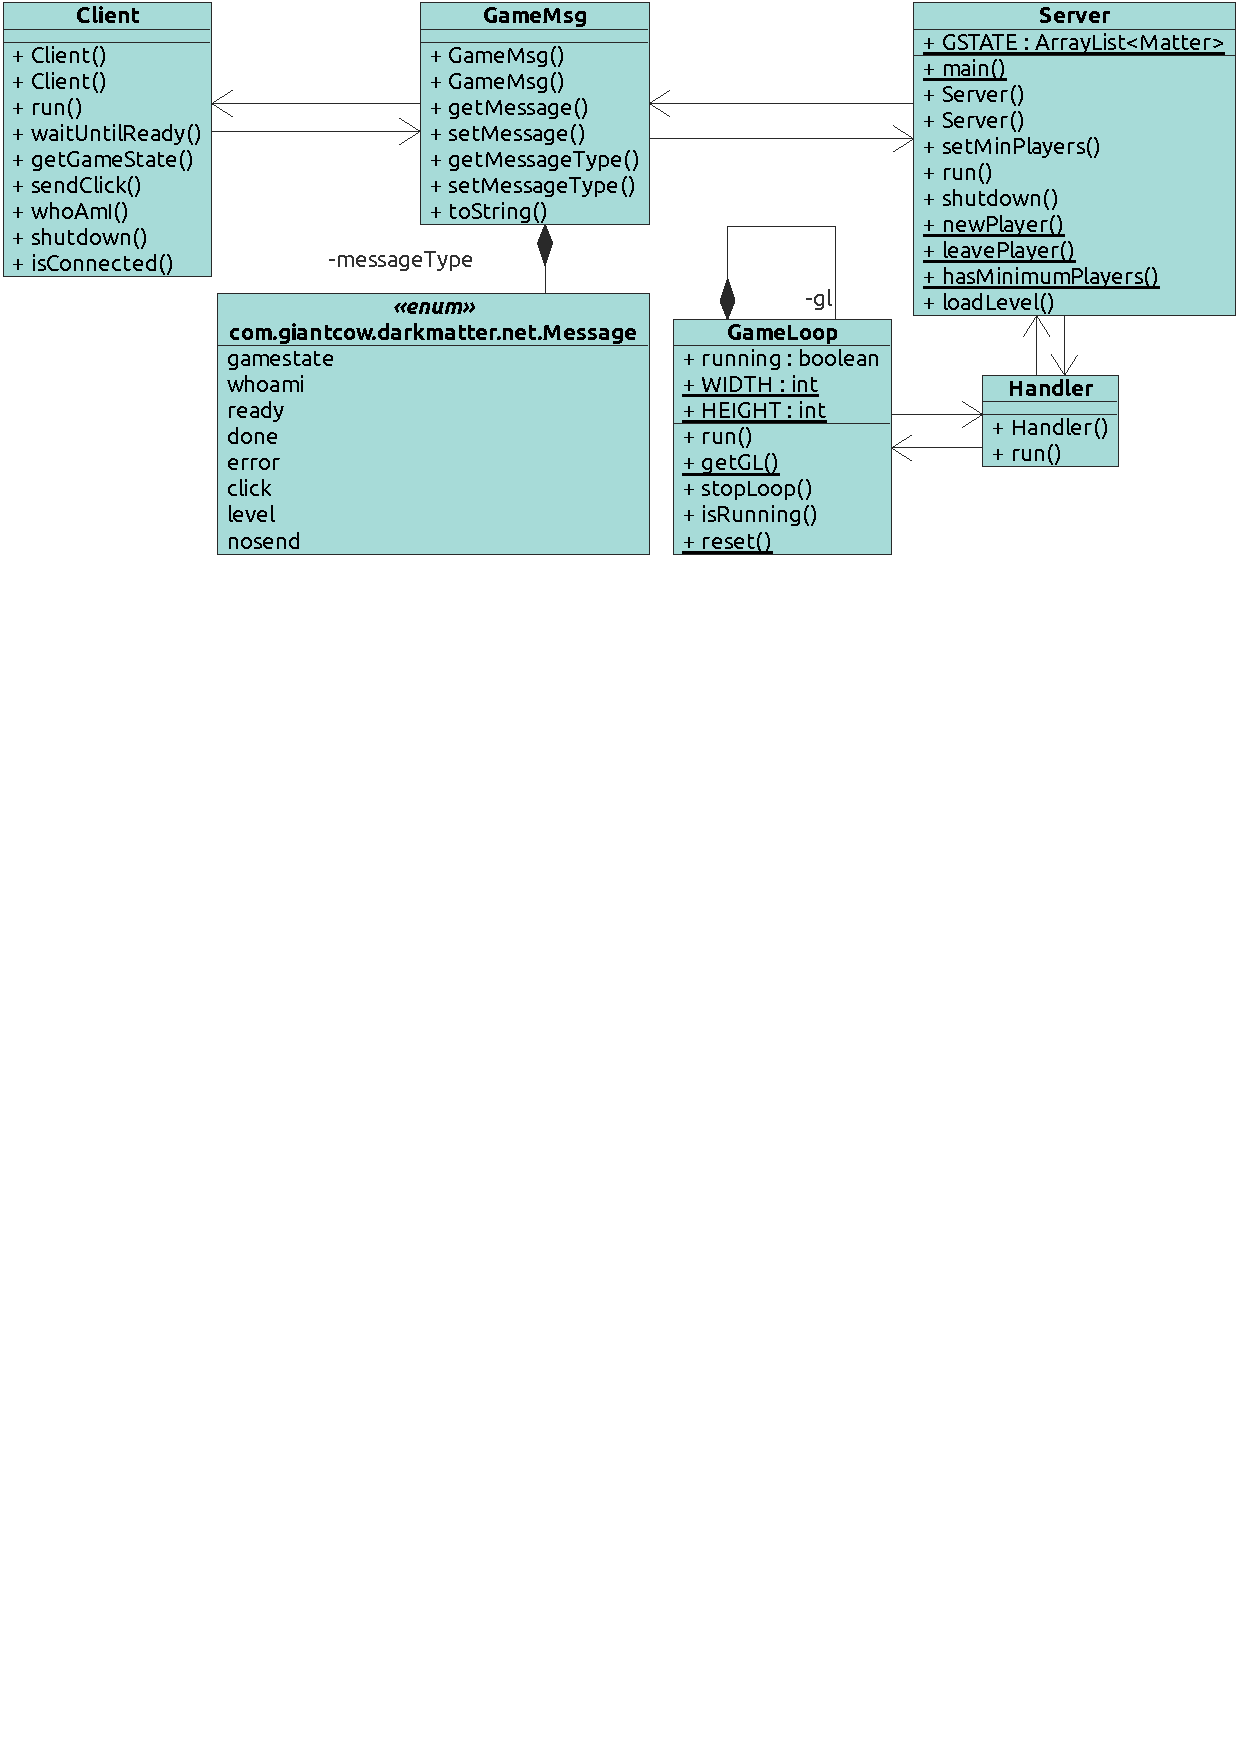
\includegraphics[width=\textwidth,trim=0 20cm 0 0]{img/network-uml.pdf}
  \caption{Networking Architecture}
  \label{fig:network_uml}
\end{figure}

The networking architecture is based on the client-server model
\cite{davison2008}. This was a relatively straightforward system to
design and implement. Our networking code places the game on the
server side of the networking stack and clients connect to it. We
chose this design, as opposed to a peer-to-peer design, because it
freed us from having to deal with synchronisation between multiple
peers.

The system we designed ended up being very flexible. There is no limit
from the server to the number of players (the max tested was six) that
can join a game. The only limiting factors are map size as well as
system resources.

Our networking architecture can be see in Figure
\ref{fig:network_uml}. The client and server can only communicate to
each other through a predefined message object. Ensuring that the two
halves of the networking stack interact in a sanitised and safe way
helped us prevent the subtle errors that arise when sending message as
Strings \cite{bloch2008}. For example, if we had encoded a message
type as a String, a simple misspelling would have caused the system to
throw and error instead of responding in the desired way.


\subsubsection{Messages}

The \texttt{GameMsg} class was a simple wrapper class. It contained
data (if needed) and a message header. The header was an \texttt{enum}
which simplified the processing code on the server side. Based on the
message header and possible data, the client or server can perform a
requested action. Figure \ref{fig:message} shows the possible
messages that could be sent.

The client begins a session by sending the \texttt{whoami}
message. This causes the server to load a \texttt{HumanMatter} object
into a game and return to the user a player number.

Clients implement a blocking wait. This means that the game would wait
and not allow anymore execution of the client-side code until there
are enough players. Accomplishing this is done with the \texttt{ready}
message. Clients simply keeping sending the message and as soon as the
server sends \texttt{true} back, client-side execution can begin
again.

\begin{wrapfigure}{r}{3cm}
  \centering
  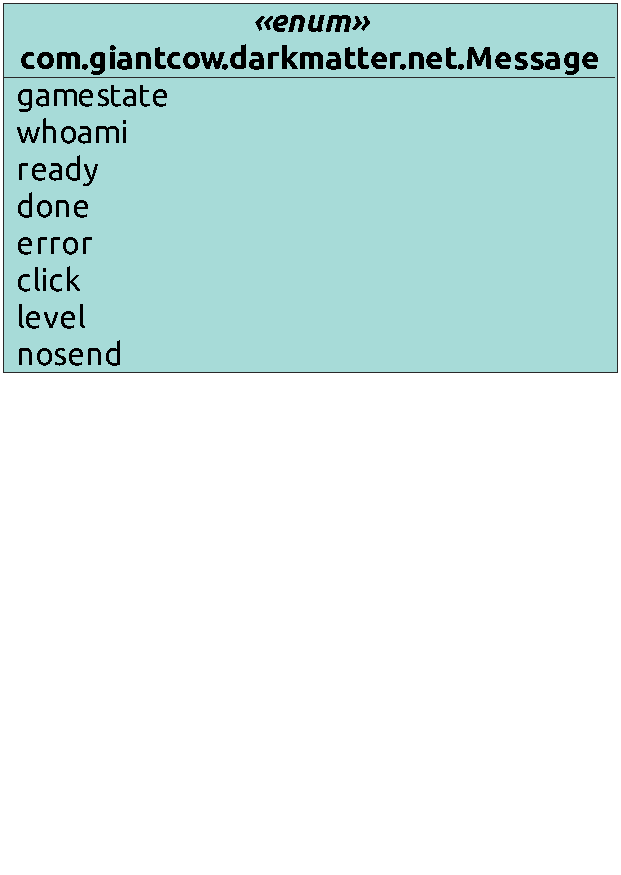
\includegraphics[width=0.3\textwidth,trim= 0 8cm 0 0]{img/message.pdf}
  \caption{The Message Protocol}
  \label{fig:message}
\end{wrapfigure}

The \texttt{gametstate} message allowed the client end to query the
server for the current state of the game. The server would then respond
in a thread-safe manner with the current state of the game.

Clients can affect the game state through the \texttt{click}
message. This is a message which contains the location of the user's
last click. The server can then use these clicks to affect how the
corresponding \texttt{Matter} objects move in the game loop.

The \texttt{level} message would request that a specified level be
loaded for game play. This was to be used to allow multiple players to
negotiate a level but due to time this feature was not implemented.

Finally the \texttt{done}, \texttt{error} and \texttt{nosend} messages
were special messages that would allow either the client or server to
deal with errors or prevent a message from being sent. The use for
these was dealing with broken connections and the end game state.


\subsubsection{Server}

All game processing happened on the server side of the networking
stack \cite{davison2008}. We wanted the server to not be tied down to
any number of players so we decided to use threads to spawn special
handlers for each client that connected. This also benefited our
system architecture because it kept separate the code to run the
server and the code to deal with client requests.

The server hosts a global variable which is shared between all client
handlers and the game loop. Allowing everyone to use the same data
structure ensured that all players were playing the same game. We
simply had to ensure that all access to the shared global variable was
thread-safe.

Additionally, the game loop ran on the server. Whenever the minimum
number of players for a type of game had been satisfied, one of the
client handlers would ensure the level was loaded into the game loop
and the begin the level. We based our game loop on the singleton
pattern \cite{gof1994}. This was a natural fit because we wanted
exactly one copy of the game loop to run on the server at a time
\cite{bloch2008}.

Rather than duplicate our code \cite{hunt1999} and have two copies of
the game loop for different modes of game play, we opted for the more
minimal approach. When the user wants to play a single player game, a
server on \texttt{localhost} was implicitly created. The user was
essentially playing a networked game for one on their own local
network. This saved us from having to maintain two branches of
identical code.


\subsubsection{Client}

Our \texttt{Client} class handles all details for the user. This class
implements the entire protocol of messages specified in Figure
\ref{fig:message}. Our aim with this class was to create a single
point of contact with the server so as to reduce its impact on the
rest of the code.

During our initial attempts at running the game in a networked
environment we were plagued with latency. The client side would query
the server for the state of the world whenever the client needed to
repaint the screen. Due to the time it took for a request to be sent
and a response to return, there was a noticeable delay in the game
(even on \texttt{localhost}).

To solve this problem we modified client to run in its own thread
\cite{horst2008:2}. While running in its thread it would be querying
the server for the game state constantly. This solved the problem of
getting the state of the game on time but it created a new one. Our
code at the time would send a message containing the location of a
click immediately after it happened. Because of this, our client code
would try and send a message while it was sending a message. Our
solution to this was to modify how clicks were sent. A user's click
were added to a queue in the client. By adding a user's click to a
queue and sending all stored clicks at a regular time, we were able to
overcome the problem of corrupting the I/O streams. Our final solution
to the problem looked roughly like Algorithm \ref{alg:client_loop}.

\begin{algorithm}                      
\caption{Client networking loop}       
\label{alg:client_loop}                
\begin{algorithmic}                    
\STATE $done \Leftarrow  false$
\WHILE{$\neg{done}$}
\STATE\COMMENT{Send all clicks added since last send}
\STATE sendClicks() 
\STATE\COMMENT{Get the new game state}
\STATE update()     
\ENDWHILE
\end{algorithmic}
\end{algorithm}


\subsection{Polish}

Creating the \emph{experience} of the game was also an important
consideration. Because of this, work to create a music player began at
the start of our development cycle. The music player was designed to
be completely decoupled from the rest of the system. Because it could
run in its own thread, we could start the music player at any point in
the code which allowed us to experiment with it while we were
developing our code. It was important to have music that gave the
right feeling and after some searching, Joss found \cite{dj_sasha} and
\cite{macleod}.

The visuals were also important for the game. Because of this we spent
a lot of time working on code to allow the user to zoom in and out on
their player. This made it so the user could navigate around cluttered
areas with ease. Since this bit of the game had no impact on the logic
of the game, it was implemented on the client's side. Each user would
want to have their own level of zoom so this makes sense. As a result
of our design decisions, the client was simply a listener for the game
state which would paint any updates that happened. The most clients
can interact is by sending a message containing the location of a
click or a request for a level to be loaded.


\section{Division of Work}

Our team had an informal approach to assigning work. As a team, we all
had our own aptitudes and desires. Fortunately, we were able to
largely assign work this way. There were only a few occasions when
multiple people wanted to work on the same component and that was
resolved quite easily.

In order to get an idea of how big everyone's contributions were, we
played the planning game. This was a useful exercise. What would
happen was that all the features for an iteration were placed on a
table. We each then estimated how long it would take us to complete
that particular feature. This was not based on an actual time value
but on the time it would take to implement a trivial feature in
Java. Our estimates would then be averaged for a final expected
time. This meant that those doing smaller features were expected to
finish earlier and then begin contributing a new feature to the code
base.


%%% Local Variables:
%%% mode: latex
%%% TeX-master: "../report"
%%% End:

% LocalWords:  refactored VelocityVector SpriteFactory gametstate UML YAML img
% LocalWords:  whoami HumanMatter localhost screenshots Yukun uml GameMsg enum
% LocalWords:  nosend sendClicks CardLayout Joss
